% THIS DOCUMENT IS FOLLOWS THE VOLERE TEMPLATE BY Suzanne Robertson and James Robertson
% ONLY THE SECTION HEADINGS ARE PROVIDED
%
% Initial draft from https://github.com/Dieblich/volere
%
% Risks are removed because they are covered by the Hazard Analysis
\documentclass[12pt]{article}

\usepackage{booktabs}
\usepackage{tabularx}
\usepackage[dvipsnames]{xcolor}
\usepackage{hyperref}
\hypersetup{
    bookmarks=true,         % show bookmarks bar?
      colorlinks=true,      % false: boxed links; true: colored links
    linkcolor=red,          % color of internal links (change box color with linkbordercolor)
    citecolor=green,        % color of links to bibliography
    filecolor=magenta,      % color of file links
    urlcolor=cyan           % color of external links
}

\newcommand{\lips}{\textit{Insert your content here.}}

%% Comments

\usepackage{color}

\newif\ifcomments\commentstrue %displays comments
%\newif\ifcomments\commentsfalse %so that comments do not display

\ifcomments
\newcommand{\authornote}[3]{\textcolor{#1}{[#3 ---#2]}}
\newcommand{\todo}[1]{\textcolor{red}{[TODO: #1]}}
\else
\newcommand{\authornote}[3]{}
\newcommand{\todo}[1]{}
\fi

\newcommand{\wss}[1]{\authornote{blue}{SS}{#1}} 
\newcommand{\plt}[1]{\authornote{magenta}{TPLT}{#1}} %For explanation of the template
\newcommand{\an}[1]{\authornote{cyan}{Author}{#1}}

%% Common Parts

\newcommand{\progname}{Software Engineering} % PUT YOUR PROGRAM NAME HERE
\newcommand{\authname}{Team 6, EcoOptimizers
\\ Nivetha Kuruparan
\\ Sevhena Walker
\\ Tanveer Brar
\\ Mya Hussain
\\ Ayushi Amin} % AUTHOR NAMES                  

\usepackage{hyperref}
    \hypersetup{colorlinks=true, linkcolor=blue, citecolor=blue, filecolor=blue,
                urlcolor=blue, unicode=false}
    \urlstyle{same}
                                


\begin{document}

\title{Software Requirements Specification for \progname: subtitle describing software} 
\author{\authname}
\date{\today}
	
\maketitle

~\newpage

\pagenumbering{roman}

\tableofcontents

~\newpage

\section*{Revision History}

\begin{tabularx}{\textwidth}{p{3cm}p{2cm}X}
\toprule {\textbf{Date}} & {\textbf{Version}} & {\textbf{Notes}}\\
\midrule
Date 1 & 1.0 & Notes\\
Date 2 & 1.1 & Notes\\
\bottomrule
\end{tabularx}

~\\

~\newpage
\section{Purpose of the Project}
\subsection{User Business}
\lips
\subsection{Goals of the Project}
\lips
\section{Stakeholders}
\subsection{Client}
The client of this project is \textbf{Dr. Istvan David} from McMaster's Department of Computing and Software. As the project supervisor, his role is to guide the development team with his technical and domain expertise. As the client, he sets the product's requirements and will be involved throughout its development. 
\subsection{Customer}
The customers of this product are all the \textbf{software developers} that use it to improve the energy efficiency of their codebase. They will be the primary users of the product and, therefore, will offer critical feedback on its effectiveness. Suggestions for improvement and/or additional features may come from this stakeholder. 

\subsection{Other Stakeholders}
\subsubsection*{\textcolor{Maroon}{Project Managers}}
They oversee project operations and focus on reducing energy costs associated with large-scale or cloud-hosted applications. They might leverage the refactoring library to reduce operational costs and achieve business sustainability goals.

\subsubsection*{\textcolor{Maroon}{Business Sustainability Teams}}
This stakeholder is responsible for reducing their company's environmental footprint by analyzing its energy emissions. They will use the energy efficiency metrics provided by the refactoring library to improve environmental sustainability practices within their organization.

\subsubsection*{\textcolor{Maroon}{End Users}}
End users refer to the users of software that uses the product in its development. They will indirectly reap benefits from these applications that have been optimised using the refactoring library. They might experience more responsive, efficient software, particularly in mobile or embedded environments where battery life is a key concern. They have no involvement in the development of the product. 

\subsubsection*{\textcolor{Maroon}{Regulatory Bodies}}
This stakeholder is responsible for establishing regulations governing energy consumption and sustainability standards. They can promote the adoption of energy-efficient software practices and potentially certify tools that meet regulatory standards. 

\subsection{Hands-On Users of the Project}
\subsubsection*{\textcolor{Maroon}{Software Developers}}
\begin{itemize}
  \item \textbf{User Role}: Integrate library into codebase, provide tests to check refactoring against original functionality

  \item \textbf{Subject Matter Experience}: Journeyman to Master
  
  \item \textbf{Technological Experience}: Journeyman to Master
  
  \item \textbf{Attitude toward technology}: Varies (conservative to positive)
  
  \item \textbf{Physical location}: Remote (at home), in-person (work office) or hybrid
\end{itemize}

\subsubsection*{\textcolor{Maroon}{Business Sustainability Teams}}
\begin{itemize}
  \item \textbf{User Role}: Access metrics provided by library

  \item \textbf{Subject Matter Experience}: Journeyman

  \item \textbf{Technological Experience}: Novice to Journeyman
  
  \item \textbf{Attitude toward technology}: Neutral to positive

\end{itemize}

\subsection{Personas}

\textbf{Persona 1} \\
Raven Reyes, a 34-year-old senior software developer, has over a decade of experience in backend development. Now working at a SaaS company focused on sustainability, Raven faces the challenge of reducing the energy consumption of their software. Manually refactoring code is time-consuming, especially when trying to pinpoint which parts of the code are draining the most energy. With tight deadlines and a need to balance sustainability with performance, Raven seeks a tool that automates energy-efficient refactoring and provides clear metrics. \\

\noindent
\textbf{Persona 2} \\
Draco Malfoy, a 29-year-old sustainability analyst at a large tech company, is tasked with reducing the environmental impact of the company’s operations. With expertise in corporate sustainability, Jordan’s role is to track and report energy consumption and carbon emissions, but they face challenges quantifying the data coming from the software development team. With the company's push toward greener technology, Jordan needs clear, easy-to-understand metrics on how the software team’s refactoring efforts are improving energy efficiency. Bridging the gap between the sustainability and development teams, Jordan relies on these insights to report progress on key sustainability goals to executives, ensuring that both technical improvements and environmental targets are aligned.

\subsection{Priorities Assigned to Users}
\textbf{Key Users:} Software Developers, Business Sustainability Teams \\
\textbf{Secondary User:} Project Managers

\subsection{User Participation}
For the bulk of the development process, requirements will be gathered from the development team itself with the help of the project supervisor, Dr. Istvan David.

During the testing phase, usability testing will be conducted to further refine the product.

\subsection{Maintenance Users and Service Technicians}
Due to the nature of this project as a capstone requirement, there are currently no expected maintenance users.

\section{Mandated Constraints}
\subsection{Solution Constraints}
\lips
\subsection{Implementation Environment of the Current System}
\lips
\subsection{Partner or Collaborative Applications}
\lips
\subsection{Off-the-Shelf Software}
\lips
\subsection{Anticipated Workplace Environment}
\lips
\subsection{Schedule Constraints}
\lips
\subsection{Budget Constraints}
\lips
\subsection{Enterprise Constraints}
\lips

\section{Naming Conventions and Terminology}
\subsection{Glossary of All Terms, Including Acronyms, Used by Stakeholders
involved in the Project}
\lips

\section{Relevant Facts And Assumptions}
\subsection{Relevant Facts}
\lips
\subsection{Business Rules}
\lips
\subsection{Assumptions}
\lips

\section{The Scope of the Work}
\subsection{The Current Situation}

  The current software development landscape often prioritizes functionality and performance over energy efficiency. Many existing Python codebases are not optimized for energy consumption, leading to unnecessary power usage and increased carbon footprint. The following aspects characterize the current situation:
  \begin{enumerate}
    \item \textbf{Manual Refactoring:} Developers typically perform refactoring manually, which is time-consuming and prone to errors.
    \item \textbf{Limited Awareness:} Many developers lack awareness of energy-efficient coding practices and their impact on overall energy consumption.
    \item \textbf{Absence of Automated Tools:} There is a lack of widely adopted automated tools specifically designed to refactor Python code for energy efficiency.
    \item \textbf{Performance-Centric Optimization:} Most existing optimization tools focus on performance improvements rather than energy efficiency.
    \item \textbf{Inefficient Code Patterns:} Many codebases contain inefficient code patterns that consume more energy than necessary.
  \end{enumerate}

  The project aims to address these issues by:
  \begin{enumerate}
    \item \textbf{Automated Refactoring Library:} Developing a Python library that automatically detects and refactors code for improved energy efficiency.
    \item \textbf{IDE Integration:} Creating a Visual Studio Code plugin that integrates the refactoring library, providing real-time suggestions and automated refactoring options.
    \item \textbf{Energy Consumption Measurement:} Implementing tools to measure and compare energy consumption before and after refactoring.
    \item \textbf{Developer Education:} Raising awareness about energy-efficient coding practices through the tool's suggestions and documentation.
    \item \textbf{Continuous Improvement:} Implementing a reinforcement learning model to improve refactoring suggestions over time based on developer feedback and real-world energy savings data.
  \end{enumerate}  

\subsection{The Context of the Work}

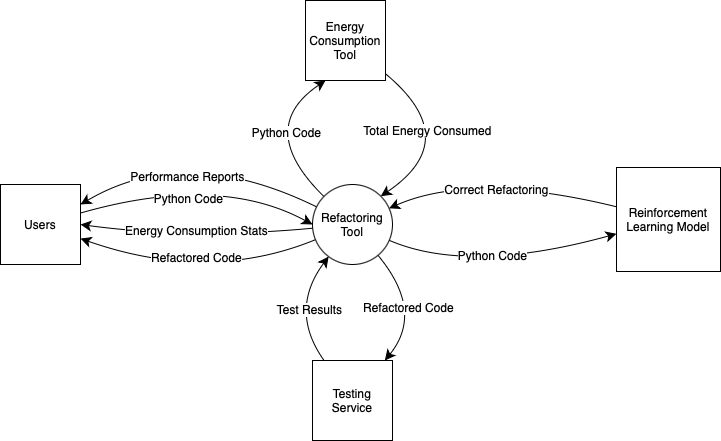
\includegraphics[scale=0.5]{../images/WorkContextModel.png}

\subsection{Work Partitioning}

\scriptsize
\begin{tabular}{ |c|p{2.5cm}|c|c| }
  \hline
  Event \# & Event Name & Input & Output(s) \\
  \hline\hline

  1 & Users submit Python code & Python Code & Refactored Code \\
  2 & Energy Analysis of code & Python Code & Total Energy Consumed \\
  3 & RI Model produces refactoring & Python Code & Correct Refactoring \\
  4 & Testing and Validation of refactored code & Refactored Code & Test Results \\
  5 & Reporting Performance metrics of new code & Refactored Code & Performance Reports \\
  6 & Viewing Energy consumption reports & Refactored Code & Energy Consumption Statistics \\

  \hline
\end{tabular}

\subsection{Specifying a Business Use Case (BUC)}

\subsubsection{Business Use Case Scenario 1}
\textbf{Event Name:} Code Submission \\
\textbf{Input:} Python Code \\
\textbf{Output:} Refactored Code \\
\textbf{Pre-condition:} User uses either GitHub Action or a VS code plugin to submit code to the refactoring tool \\  
\textbf{Scenario:}
    \begin{enumerate}
        \item Refactoring tool receives the Python code
        \item PyJoules is used to store energy consumption data for original Python code submitted
        \item Tool analyzes the code for inefficiencies (PySmells)
        \item Python code is provided to Re-enforcement learning model to find a refactoring
        \item Energy consumption is measured of refactored code and compared to the original data
        \item Refactored code is tested to ensure functionality is maintained from original code
        \item Refactored code is received by the user
    \end{enumerate}
\textbf{Sub Variation: }
    \begin{itemize}
        \item \textit{4a:} If no PySmells identified, then code is returned to the user
        \item \textit{6a:} If energy consumption increases for refactored code, the reinforcement model is asked to find another refactoring
        \item \textit{7a:} If code functionality is not preserved for refactored code, the reinforcement model is asked to find another refactoring
    \end{itemize}

\subsubsection{Business Use Case Scenario 2} 
\textbf{Event Name:} Energy Analysis of Code \\
\textbf{Input:} Python Code \\
\textbf{Output:} Total Energy Consumed \\
\textbf{Pre-condition:} Submission of Python code to the Energy Consumption Tool \\
\textbf{Scenario: } 
\begin{itemize}
    \item \textit{1:} Tool receives Python Code
    \item \textit{2:} Energy consumed is measured during execution
    \item \textit{3:} The analysis results are compiled into a report
    \item \textit{4:} Report of total energy consumed is received by the refactoring tool
\end{itemize}

\subsubsection{Business Use Case Scenario 3} 
\textbf{Event Name:} Reinforcement Learning Model Produces Refactoring \\
\textbf{Input:} Python Code \\
\textbf{Output:} Correct Refactoring \\
\textbf{Pre-condition:} Request for refactored code from the Reinforcement Learning Model \\
\textbf{Scenario: } 
\begin{itemize}
    \item \textit{1:} Model receives Python Code
    \item \textit{2:} Analyze Code for potential refactoring
    \item \textit{3:} Generate suggestions based on previous learning and data
    \item \textit{4:} Implement suggested refactorings
\end{itemize}
\textbf{Sub Variation: }
\begin{itemize}
    \item \textit{2a:} If there are no refactorings found, Model outputs given code back to the refactoring tool 
\end{itemize}

\subsubsection{Business Use Case Scenario 4} 
\textbf{Event Name:} Testing and Validation of Refactored Code \\
\textbf{Input:} Refactored Code \\
\textbf{Output:} Test Results \\
\textbf{Pre-condition:} Energy consumed for refactored code is less than energy consumed for original code \\
\textbf{Scenario: } \\
\begin{itemize}
    \item \textit{1:} Conduct tests on refactored code
    \item \textit{2:} Conduct tests on original code
    \item \textit{3:} Validate results of refactored code to the results of the original code to ensure functionality is intact
    \item \textit{4:} Signal to refactoring tool to send refactored code to user
\end{itemize}
\textbf{Sub Variation: }
\begin{itemize}
    \item \textit{4a:} If functionality is not preserved, signal to the refactoring tool to refactor again
\end{itemize}

\subsubsection{Business Use Case Scenario 5} 
\textbf{Event Name:} Reporting Performance Metrics of New Code \\
\textbf{Input:} Refactored Code \\
\textbf{Output:} Performance Reports\\
\textbf{Pre-condition:} Testing and validation is completed successfully \\
\textbf{Scenario: } \\
\begin{itemize}
    \item \textit{1:} Generate detailed performance report based on testing outcomes
    \item \textit{2:} User receives the performance report
\end{itemize}

\subsubsection{Business Use Case Scenario 6} 
\textbf{Event Name:} Viewing Energy Consumption Reports \\
\textbf{Input:} Refactored Code \\
\textbf{Output:} Energy Consumption Statistics \\
\textbf{Pre-condition:} Testing and validation is completed successfully \\
\textbf{Scenario: } \\
\begin{itemize}
    \item \textit{1:} Comprehensive statistics are compiled from energy analysis data
    \item \textit{2:} Information is compiled in an accessible format for developers to review
\end{itemize}


\section{Business Data Model and Data Dictionary}
\subsection{Business Data Model}
\lips
\subsection{Data Dictionary}
\lips

\section{The Scope of the Product}
\subsection{Product Boundary}
\lips
\subsection{Product Use Case Table}
\lips
\subsection{Individual Product Use Cases (PUC's)}
\lips

\section{Functional Requirements}
\subsection{Functional Requirements}
\lips

\section{Look and Feel Requirements}
\subsection{Appearance Requirements}
\lips
\subsection{Style Requirements}
\lips

\section{Usability and Humanity Requirements}
\subsection{Ease of Use Requirements}
\lips
\subsection{Personalization and Internationalization Requirements}
\lips
\subsection{Learning Requirements}
\lips
\subsection{Understandability and Politeness Requirements}
\lips
\subsection{Accessibility Requirements}
\lips

\section{Performance Requirements}
\subsection{Speed and Latency Requirements}
\lips
\subsection{Safety-Critical Requirements}
\lips
\subsection{Precision or Accuracy Requirements}
\lips
\subsection{Robustness or Fault-Tolerance Requirements}
\lips
\subsection{Capacity Requirements}
\lips
\subsection{Scalability or Extensibility Requirements}
\lips
\subsection{Longevity Requirements}
\lips

\section{Operational and Environmental Requirements}
\subsection{Expected Physical Environment}
\lips
\subsection{Wider Environment Requirements}
\lips
\subsection{Requirements for Interfacing with Adjacent Systems}
\lips
\subsection{Productization Requirements}
\lips
\subsection{Release Requirements}
\lips

\section{Maintainability and Support Requirements}
\subsection{Maintenance Requirements}
\begin{enumerate}
  \item \textbf{Requirement:} The tool must allow new refactoring techniques to be added within one week of identification.
     \begin{itemize}
         \item \textbf{Rationale:} Rapid integration of new techniques ensures the tool remains up-to-date with evolving best practices in energy-efficient coding.
         \item \textbf{Fit Criteria:} Developers can integrate new refactoring methods into the tool, and they are fully operational within seven days.
     \end{itemize}
     
  \item \textbf{Requirement:} The tool must be maintainable by developers who are not the original creators.
     \begin{itemize}
         \item \textbf{Rationale:} Ensuring that new developers can easily understand and modify the system reduces dependency on original developers and facilitates long-term maintenance.
         \item \textbf{Fit Criteria:} Comprehensive documentation is available, including setup guides and code comments, allowing new developers to understand and modify the system within two days.
     \end{itemize}
     
  \item \textbf{Requirement:} The tool must allow for easy rollback of updates in case of errors.
     \begin{itemize}
         \item \textbf{Rationale:} Quick rollback capabilities minimize downtime and user disruption in case an update introduces issues.
         \item \textbf{Fit Criteria:} Any update can be reverted with minimal effort, ensuring the system returns to a stable state within one hour.
     \end{itemize}
     
  \item \textbf{Requirement:} The tool must provide automated testing for all refactoring functions.
     \begin{itemize}
         \item \textbf{Rationale:} Automated testing ensures that changes do not introduce new bugs, maintaining the reliability and stability of the tool.
         \item \textbf{Fit Criteria:} All refactoring methods have associated unit tests that run automatically with each code change, ensuring 80\% code coverage.
     \end{itemize}
     
  \item \textbf{Requirement:} Each version of the library must maintain compatibility with the current releases of external libraries during its development phase. .
     \begin{itemize}
         \item \textbf{Rationale:} Keeping external libraries up-to-date ensures compatibility and leverages improvements or security patches provided by library maintainers.
         \item \textbf{Fit Criteria:} The system successfully integrates updates from external libraries without breaking existing functionality.
     \end{itemize}
  
  \end{enumerate}

\subsection{Supportability Requirements}
\begin{enumerate}
  \item \textbf{Requirement:} The tool must offer bilingual support for help documentation.
  \begin{itemize}
      \item \textbf{Rationale:} Bilingual support ensures that users from different regions can understand and use the tool effectively, increasing its accessibility.
      \item \textbf{Fit Criteria:} Help documentation is available in both major languages, English and French.
  \end{itemize}
  
\end{enumerate}

\subsection{Adaptability Requirements}
Not applicable in this project currently

\section{Security Requirements}
\subsection{Access Requirements}
\lips
\subsection{Integrity Requirements}
\lips
\subsection{Privacy Requirements}
\lips
\subsection{Audit Requirements}
\lips
\subsection{Immunity Requirements}
\lips

\section{Cultural Requirements}
\subsection{Cultural Requirements}
\lips

\section{Compliance Requirements}
\subsection{Legal Requirements}
\lips
\subsection{Standards Compliance Requirements}
\lips

\section{Open Issues}
\lips

\section{Off-the-Shelf Solutions}
\subsection{Ready-Made Products}
\lips
\subsection{Reusable Components}
\lips
\subsection{Products That Can Be Copied}
\lips

\section{New Problems}
\subsection{Effects on the Current Environment}
\lips
\subsection{Effects on the Installed Systems}
\lips
\subsection{Potential User Problems}
\lips
\subsection{Limitations in the Anticipated Implementation Environment That May
Inhibit the New Product}
\lips
\subsection{Follow-Up Problems}
\lips

\section{Tasks}
\subsection{Project Planning}
\begin{itemize}
 
  \item \textbf{Development Approach}
  The team will use an agile development approach with the following high-level process:
  \begin{enumerate}
    \item Initial requirements gathering and product backlog creation
    \item Sprint planning and execution
    \item Regular testing and quality assurance
    \item Stakeholder reviews and feedback
    \item Iterative refinement
    \item Release planning and deployment
  \end{enumerate}
  
 \item \textbf{Key Tasks}
  \begin{itemize}
    \item Form cross-functional development team (already completed) 
    \item Create initial product backlog and prioritize features
    \item Set up development environments and tools
    \item Establish CI/CD pipeline using GitHub Actions
    \item Develop core functionality:
      \begin{itemize}
        \item Determine code smells to address for energy saving
        \item Implement code smell detection
        \item Develop appropriate refactorings for detected smells
        \item Measure energy consumption before and after refactoring
        \item Ensure original code functionality is preserved
      \end{itemize}
    \item Build out additional features iteratively
    \item Conduct regular testing (unit, integration, user acceptance)
    \item Refine based on stakeholder feedback
    \item Present final solution to stakeholders

  \end{itemize}
  \item \textbf{Timeline Estimate}
    \begin{itemize}
        \item Requirements Document (Revision 0): October 9th, 2024
        \item Hazard Analysis (Revision 0): October 23rd, 2024
        \item Verification \& Validation Plan (Revision 0): November 1st, 2024
        \item Proof of Concept: November 11th-22nd, 2024
        \item Design Document (Revision 0): January 15th, 2025
        \item Project Demo (Revision 0): February 3rd-14th, 2025
        \item Final Demonstration: March 17th-30th, 2025
        \item Final Documentation: April 2nd, 2025
        \item Capstone EXPO: TBD
    \end{itemize}
    
  \item \textbf{Resource Estimates}
  The team consists of 5 members who will all function as developers, sharing responsibilities for creating issues, coding, testing, and documentation.

  \item \textbf{Key Consideration}
    \begin{itemize}
        \item Data migration may be necessary for existing systems
        \item A phased development approach will help minimize major setbacks
        \item Regular stakeholder involvement will ensure alignment with business needs
    \end{itemize}

  \item \textbf{Documentation Process}
    \begin{itemize}
        \item Pull changes from \texttt{docs} (epic documentation branch)
        \item Create working branch with format [main contributor name]/[descriptive topic]
        \item Commit changes with descriptive names
        \item Create unit tests for changes
        \item Create pull request to merge changes into epic branch
        \item Wait for all tests run with GitHub Actions to pass
        \item Wait for at least two approvals from teammates
        \item Merge changes into target branch
    \end{itemize}
  
\end{itemize}

By following this agile approach and development process, the team aims to deliver a high-quality product iteratively while maintaining flexibility to adapt to changing requirements

\subsection{Planning of the Development Phases}

The planning of the development phases is based on the deliverables submissions as follows:

\begin{enumerate}

    \item \textbf{Requirements Phase}
    \begin{itemize}
        \item Deliverable: Requirements Document (Revision 0)
        \item Due Date: October 9th, 2024
    \end{itemize}
    
    \item \textbf{Risk Assessment Phase}
    \begin{itemize}
        \item Deliverable: Hazard Analysis (Revision 0)
        \item Due Date: October 23rd, 2024
    \end{itemize}
    
    \item \textbf{Verification and Validation Planning}
    \begin{itemize}
        \item Deliverable: Verification \& Validation Plan (Revision 0)
        \item Due Date: November 1st, 2024
    \end{itemize}
    
    \item \textbf{Proof of Concept Implementation}
    \begin{itemize}
        \item Period: November 11th-22nd, 2024
    \end{itemize}
    
    \item \textbf{Design Phase}
    \begin{itemize}
        \item Deliverable: Design Document (Revision 0)
        \item Due Date: January 15th, 2025
    \end{itemize}
    
    \item \textbf{Initial Implementation and Demo}
    \begin{itemize}
        \item Deliverable: Project Demo (Revision 0)
        \item Period: February 3rd-14th, 2025
    \end{itemize}
    
    \item \textbf{Final Implementation and Testing}
    \begin{itemize}
        \item Deliverable: Final Demonstration
        \item Period: March 17th-30th, 2025
    \end{itemize}
    
    \item \textbf{Project Closure}
    \begin{itemize}
        \item Deliverable: Final Documentation
        \item Due Date: April 2nd, 2025
    \end{itemize}
    
    \item \textbf{Project Presentation}
    \begin{itemize}
        \item Event: Capstone EXPO
        \item Date: TBD
    \end{itemize}
\end{enumerate}


\section{Migration to the New Product}
\subsection{Requirements for Migration to the New Product}
\lips
\subsection{Data That Has to be Modified or Translated for the New System}
\lips

\section{Costs}
\lips
\section{User Documentation and Training}
\subsection{User Documentation Requirements}
\lips
\subsection{Training Requirements}
\lips

\section{Waiting Room}
\lips

\section{Ideas for Solution}
\lips

\newpage{}
\section*{Appendix --- Reflection}

The information in this section will be used to evaluate the team members on the
graduate attribute of Lifelong Learning.  Please answer the following questions:

\begin{enumerate}
  \item What knowledge and skills will the team collectively need to acquire to
  successfully complete this capstone project?  Examples of possible knowledge
  to acquire include domain specific knowledge from the domain of your
  application, or software engineering knowledge, mechatronics knowledge or
  computer science knowledge.  Skills may be related to technology, or writing,
  or presentation, or team management, etc.  You should look to identify at
  least one item for each team member.
  \item For each of the knowledge areas and skills identified in the previous
  question, what are at least two approaches to acquiring the knowledge or
  mastering the skill?  Of the identified approaches, which will each team
  member pursue, and why did they make this choice?
\end{enumerate}

\end{document}
